\chapter{Published models}

This chapter will present five publicly available job scheduling models based on deep reinforcement learning on graph neural networks. Three models are designed for JSSP, and two are for FJSP. For models designed for JSSP, our extension to JSSP is also presented. Each presented model is named after the GitHub repository in which it was found. 

\section{JSSP Models}

\subsection{L2D}
\textbf{L2D} is a model published in \cite{zhang2020learning}, source code was obtained from \cite{github_l2d}. To represent the JSSP, it employs a modified disjunctive graph described in \ref{JSSP as a disjunctive graph}, where the authors start with the original disjunctive graph containing only conjunctive arcs, and after each dispatched operation, they add a conjunctive arc representing new precedence constraint. This process is shown in the Figure 3.1 below \cite{zhang2020learning}. This design solves the problem: replacing each disjunctive edge with a pair of opposite conjunctive arcs results in a too-dense, fully oriented graph \cite{zhang2020learning}.
\par
To parametrize the policy $\pi_\theta(a_t|s_t)$, GIN for oriented graphs described in \ref{graph Isomorphism network} is used to obtain graph node embeddings $\vec{h}_o^{(K)}$ in the message passing phase. Initial node features were a 2-elementer vector $\vec{h}_o^{(0)} = (I(o), C_{LB}(o))$, where $I(o)$ is equal to 1 only if $o \in O$ is scheduled, otherwise 0, and $C_{LB}(o)$ is the lower bound of the estimated time of completion. 
\par
To select the action $a_t$ at $s_t$ in the readout phase, obtained graph embeddings are pooled using average pooling, i.e., $\vec{h}_G = \frac{1}{|O|} \sum_{o \in O} \vec{h}_o^{(K)}$, concatenated with the embedding of the eligible operation $o$ corresponding to the action $a_t$, and passed through a multi-layer perceptron to obtain a score for the corresponding action $scr(a_t) = \text{MLP}_{\pi_\theta}\left ( \left [h_o^{(T)} || h_G \right ] \right )$. The softmax function is then applied to obtain a distribution over available actions $P(a_t)$ from the scores \cite{zhang2020learning}. Selected action is started as soon as possible. To train the policy, authors used PPO discussed in \ref{policy_optimization}.
\begin{center}
    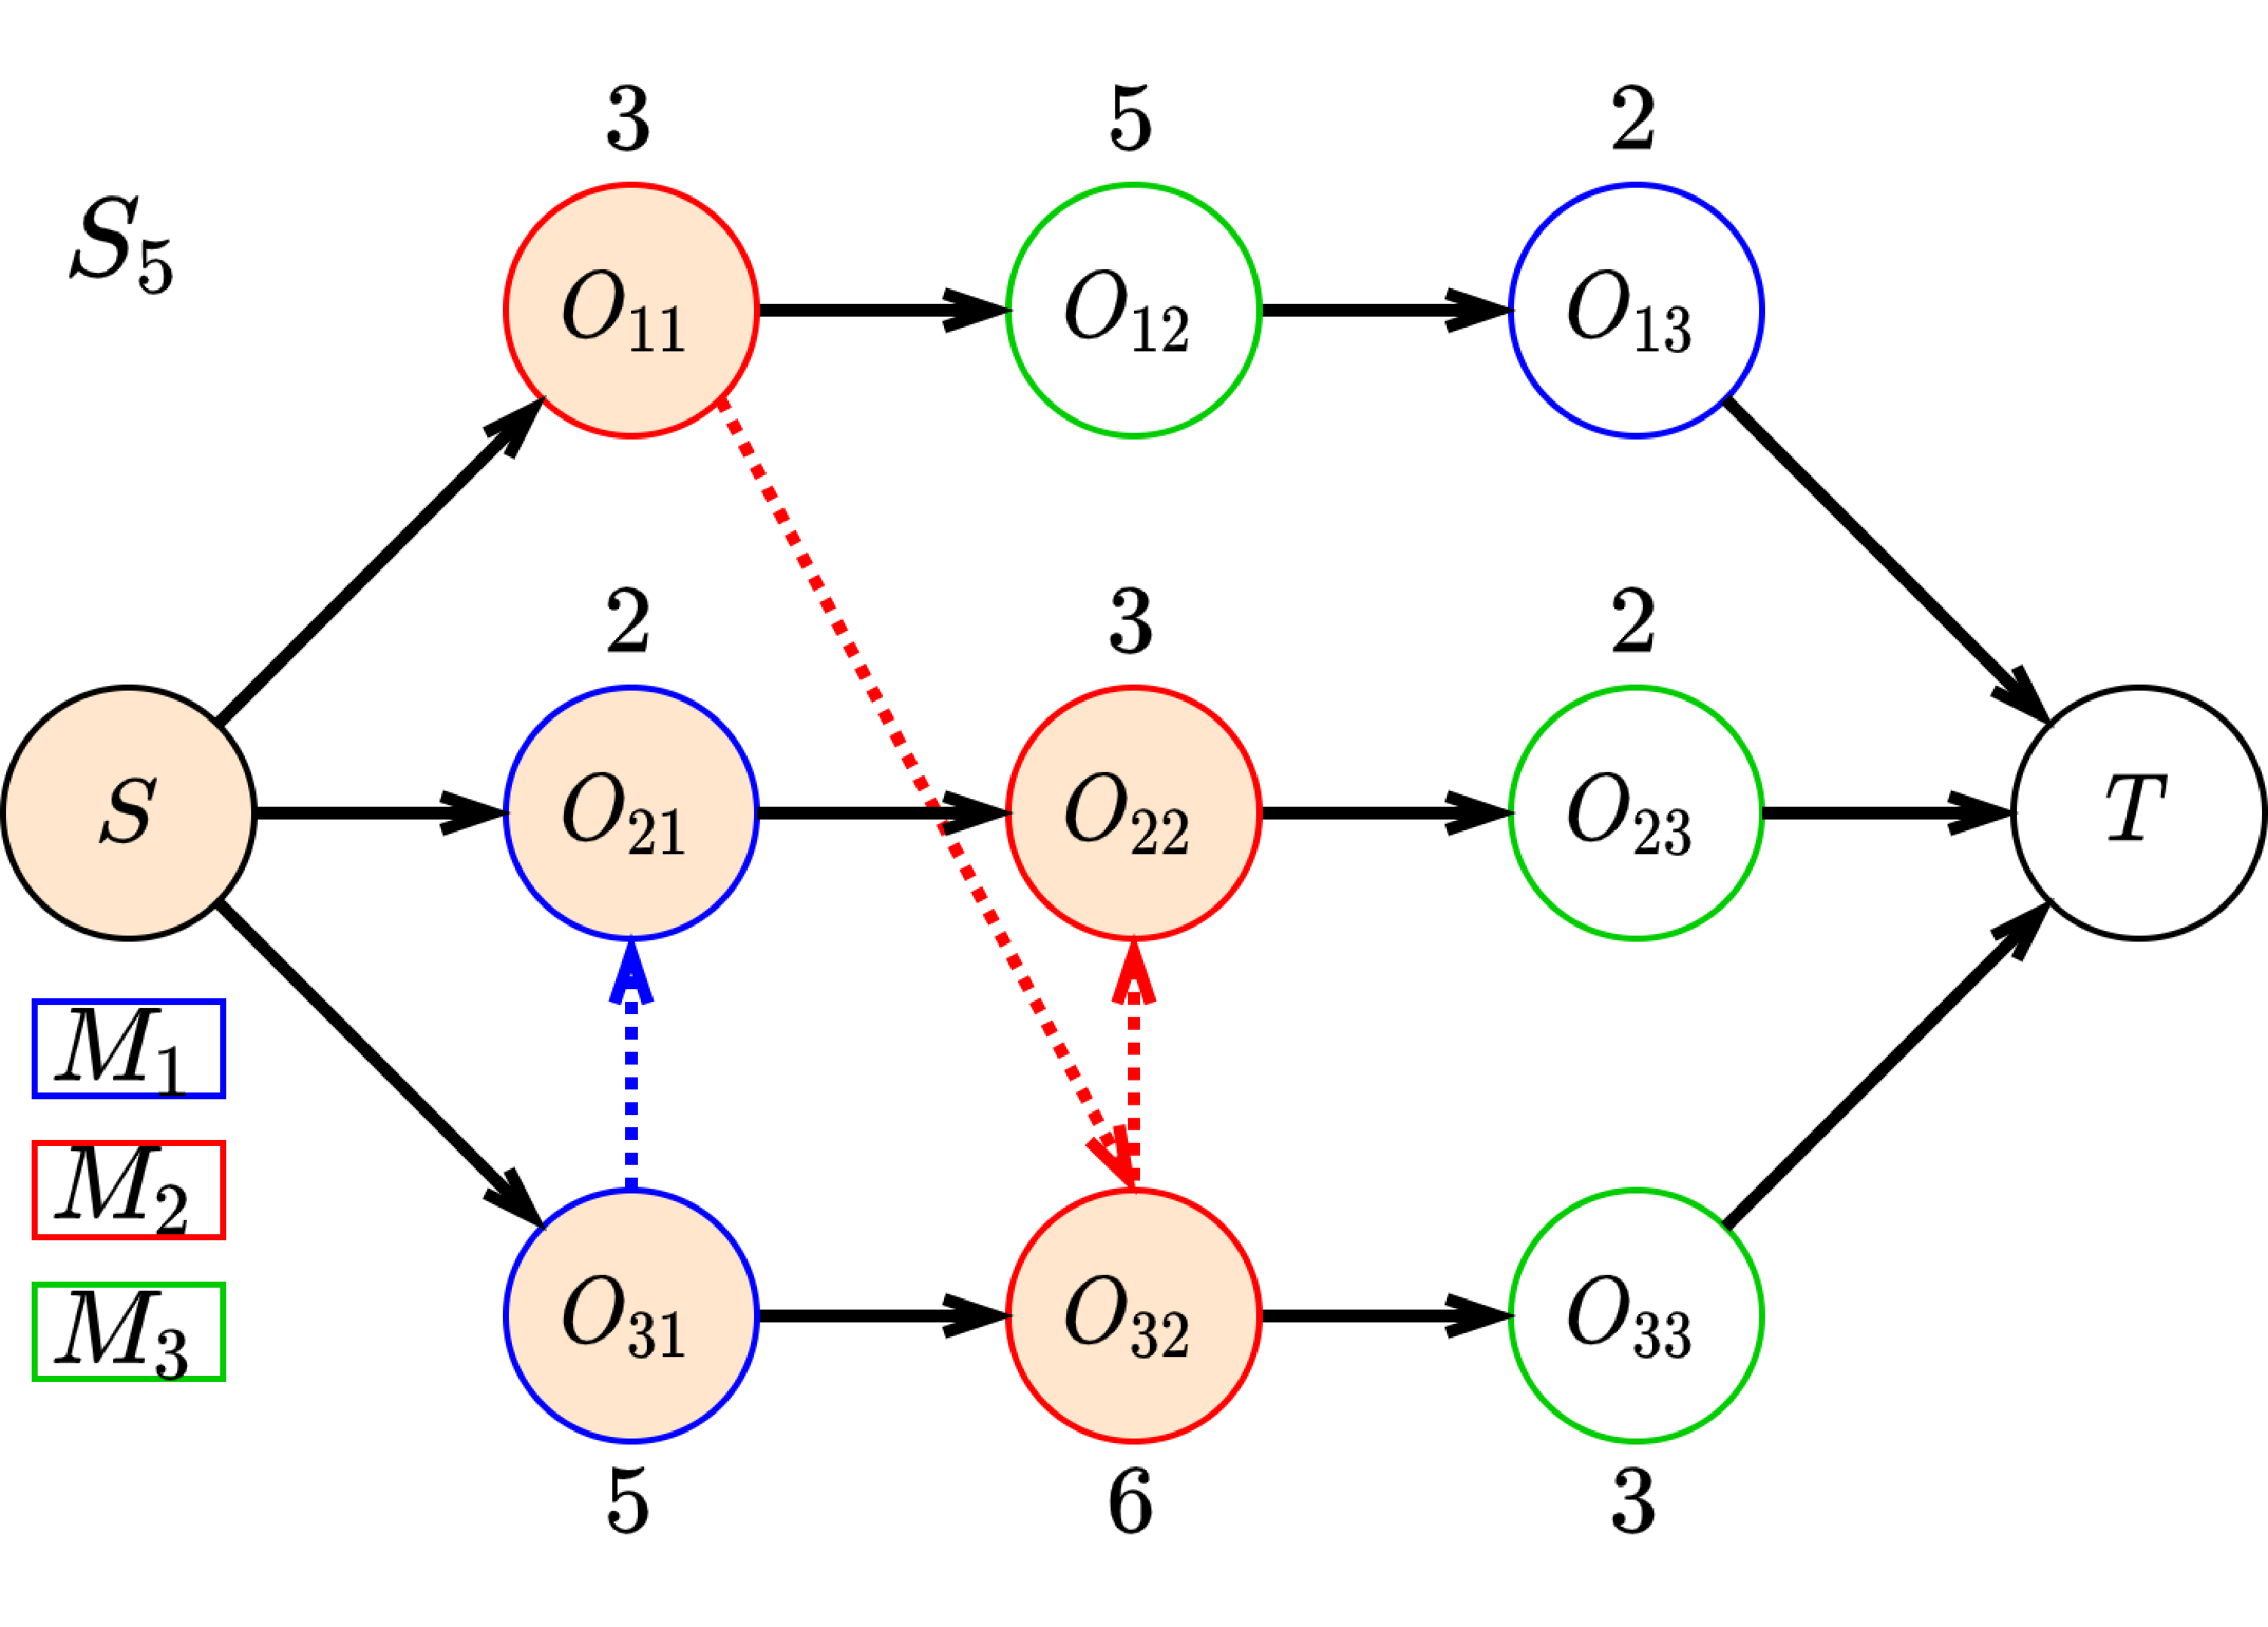
\includegraphics[width=0.75\linewidth]{images/jssp_adding_arcs.pdf}\\
    Figure 3.1: \textit{"Adding arc strategy"}: Disjunctive graph with original precedence constraints (black arrows), and three precedence constraints (red and blue arrows) between already scheduled operations (orange circles). Retrieved from \cite{zhang2020learning}.
\end{center}

\subsubsection{Dynamic L2D}

Since \textbf{L2D} is a model developed strictly for JSSP, we had to extend it to apply to DJSP. The main idea behind our algorithm is that when a new job $J_\text{new}$ arrives with the arrival time $t_a$, we want to reschedule all operations that have not started yet. To do this, we keep track of currently known jobs $J_\text{known}$, and a list of already started operations ($S_{ij} < t_a$) called \textit{plan}. When rescheduling, we first formulate the JSSP instance from known jobs and dispatch operations from the plan. By doing this, we get a partially solved JSSP with all operations with $S_{ij} \geq t_a$ removed. Then, we let \textbf{L2D} select operations to dispatch and enforce the lower bound for start time $S_{ij} \geq  t_a$. We repeat this until some termination criteria are not met, for example, no new jobs are expected. This algorithm, written in pseudocode, is shown below.

\begin{algorithm}[H]
	\caption{Dynamic L2D}\label{algorithm:dqn}
	\begin{algorithmic}
	\State $J_\text{known} \gets$ jobs known at the start
    \State $plan \gets$ initialize empty list of actions 
    \State $instance \gets$ formulate JSSP instance from $J_\text{known}$
    \State $solution \gets$ dispatch operations in $instance$ with \textbf{L2D} 
	\While{termination criteria not met}
        \State $J_\text{new} \gets$ check if new job arrived
        \If{$J_\text{new} = \emptyset$}
            \State \textbf{continue}
        \EndIf
		\For{operation $O_{ij}$ in $solution$}
            \If{$S_{ij} < t_a$ and $O_{ij}$ not in $plan$}
                \State add $O_{ij}$ to the $plan$
            \EndIf
		\EndFor
        \State add $J_\text{new}$ to $J_\text{known}$
        \State $instance \gets$ formulate JSSP instance from $J_\text{known}$
        \For{operation $O_{ij}$ in $plan$}
            \State dispatch $O_{ij}$ in $instance$
        \EndFor
        \State $solution \gets$ dispatch the rest of $instance$ with \textbf{L2D} and constraint $S_{ij} \geq t_a$ 
	\EndWhile
    \State return $solution$
\end{algorithmic}
\end{algorithm}

\subsection{IEEE-ICCE-RL-JSP}

\textbf{IEEE-ICCE-RL-JSP} was published in \cite{10226873}, code was obtained from Github repository \cite{github_ieee_icce_rl_jsp}. Authors represent JSSP as a heterogeneous graph discussed in \ref{FJSP as a heterogenous graph}. In each step, this model chooses one of the traditional PDRs to determine the operation to dispatch.
\par
To parametrize the policy, authors used GIN on heterogeneous graphs discussed in \ref{graph Isomorphism network} in the message passing phase. Features of operation nodes include the status of the operation, the processing time, the remaining time of the operation, and the number of remaining operations in the current job. Features of machine nodes include the status of the corresponding machine and the remaining time of the operation being processed \cite{10226873}.
\par
In the readout phase, obtained embeddings are pooled using sum pooling and fed into a value network based on DDQN discussed in \ref{dqn}, which outputs a score value for each PDR. The agent selects a PDR with a maximum score to determine which operation to dispatch \cite{10226873}.

\subsubsection{Dynamic IEEE-ICCE-RL-JSP}

After the inspection of the source code \cite{github_ieee_icce_rl_jsp} published in \cite{10226873}, we discovered that the authors already had prepared the functionality for setting the arrival time of the job, but it was not described in the paper itself \cite{10226873}. Therefore, we only needed to modify the source code to be able to pass job arrival times to the model. 
\par
\textbf{IEEE-ICCE-RL-JSP} takes a list of jobs and their arrival times as an input. When the model chooses which operation to dispatch, operations from jobs that have not yet arrived are not listed as eligible operations, i.e., job arrival time $t_a$ is greater than the current time.

\section{FJSP Models}

\subsection{End-to-end-DRL-for-FJSP} 

\textbf{End-to-end-DRL-for-FJSP} was published in \cite{LEI2022117796}, source code was obtained from \cite{github_end_to_end_drl_for_fjsp}. Authors represented FJSP as a disjunctive graph discussed in \ref{FJSP as a disjunctive graph}. To reduce the computational complexity, authors used the \textit{"adding arc scheme"} similar to authors of \textbf{L2D}. This process for FJSP is shown in Figure 3.2 below.
\begin{center}
    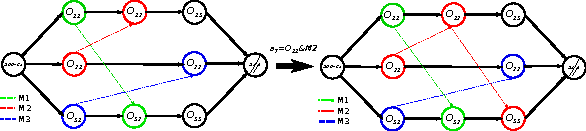
\includegraphics[width=\linewidth]{images/fjsp_adding_arcs.pdf}\\
    Figure 3.2: \textit{"Adding arc strategy"} for FJSP: Disjunctive graph with original precedence constraints (black arrows) between unscheduled operations (black circles), and three precedence constraints (red and blue arrows) between already scheduled operations (colorful circles). Action $a_7$ dispatches operation $O_{33}$ on machine $M2$ by adding a red arc corresponding to machine $M2$ and changing the color of operation $O_{33}$ to red. Retrieved from \cite{LEI2022117796}.
\end{center}
In the message passing phase, authors use GIN discussed in \ref{graph Isomorphism network}. Extracted operation node embeddings $\vec{h}_o^{(K)}$ are pooled using average pooling $\vec{h}_G = \frac{1}{|O|} \sum_{o \in O} \vec{h}_o^{(K)}$ as in \textbf{L2D}. Input features of each operation node are the same as in \textbf{L2D}, i.e., $\vec{h}_o^{(0)} = (I(o), C_{LB}(o))$, where $I(o)$ is equal to 1 only if $o \in O$ is scheduled, otherwise 0, and $C_{LB}(o)$ is the lower bound of the estimated time of completion.
\par
Resulting operation node embeddings do not include machine information. Authors adopt a fully connected layer to encode the machine's state to counteract this. Machine embeddings $\vec{h}_m$ are then pooled to obtain a machine pooling vector $\vec{u}_m$. 
\par
To select the action in the readout phase, two decoders based on multi-layer perceptron with the same structure. Each decoder computes a probability distribution over the operation and machine space, respectively. In the first step, each decoder computes an operation score $c_o$ and machine score $c_m$ \cite{LEI2022117796}
\begin{equation}
    c_o = \text{MLP}_{\pi_{\theta}(o)} \left ( \vec{h}_o^{(K)} || \vec{h}_G || \vec{u}_m \right ) \hspace{2em} \forall o \in O \, ,
\end{equation}
\begin{equation}
    c_m = \text{MLP}_{\pi_{\theta}(m)} \left ( \vec{h}_m^{(T)} || \vec{h}_G || \vec{u}_m \right ) \hspace{2em} \forall m \in \mathcal{M} \, .
\end{equation}
